\begin{correction}   \;
\begin{enumerate}
\item Soit $m\in\R^{\star}$ fix\'e. La fonction $f_m$ est bien d\'efinie si et seulement si: $1+x>0\Leftrightarrow x>-1$ et ainsi $\mathcal{D}_{f_m}=\rbrack -1,+\infty\lbrack$.
\item
\begin{itemize}
\item[$\bullet$] Limite en $-1$: par propri\'et\'e sur les somme, compos\'ee et produit de limite $\lim\limits_{x\to -1^+} x\ln{(1+x)}=+\infty$. Ainsi on doit distinguer deux cas selon que $m>0$ ou $m<0$.
\begin{itemize}
\item[$\star$] Si $m>0$, alors $\lim\limits_{x\to -1^+} f_m(x)=+\infty$ par propri\'et\'e sur les produit et compos\'ee de limite.
\item[$\star$] Si $m<0$, alors $\lim\limits_{x\to -1^+} f_m(x)=0$ par propri\'et\'e sur les produit et compos\'ee de limite.
\end{itemize}
\item[$\bullet$] Limite en $+\infty$: par propri\'et\'e sur les somme, compos\'ee et produit de limite $\lim\limits_{x\to+\infty} x\ln{(1+x)}=+\infty$. Ainsi on doit distinguer deux cas selon que $m>0$ ou $m<0$.
\begin{itemize}
\item[$\star$] Si $m>0$, alors $\lim\limits_{x\to +\infty} f_m(x)=+\infty$ par propri\'et\'e sur les produit et compos\'ee de limite.
\item[$\star$] Si $m<0$, alors $\lim\limits_{x\to +\infty} f_m(x)=0$ par propri\'et\'e sur les produit et compos\'ee de limite.
\end{itemize}
\end{itemize}
\item  Soit $m\in\R^{\star}$ fix\'e. La fonction $f_m$ est d\'erivable sur $\rbrack -1,+\infty\lbrack$ comme somme, compos\'ee et produit de limite. De plus, on a, pour tout $x>-1$: 
$$f_m^{\prime}(x)=e^{mx\ln{(1+x)}} \left(  m\ln{(1+x)} +\ddp\frac{mx}{1+x}  \right)=m e^{mx\ln{(1+x)}} \left(  \ln{(1+x)} +\ddp\frac{x}{1+x}  \right)=mf_m(x)g_m(x) $$
avec $g_m(x)= \ln{(1+x)} +\ddp\frac{x}{1+x}  $.
\item Comme on ne sait pas \'etudier le signe de $g_m$ directement, on \'etudie les variations de cette fonction pour en d\'eduire son signe. 
\begin{itemize}
\item[$\bullet$] La fonction $g_m$ est d\'erivable sur $\rbrack -1,+\infty\lbrack$ comme compos\'e, quotient et somme de fonctions d\'erivables. De plus, pour tout $x>-1$, on a: $g_m^{\prime}(x)=\ddp\frac{1}{1+x} +\ddp\frac{1}{(1+x)^2}=\ddp\frac{2+x}{(1+x)^2} $. 
\item[$\bullet$] On en d\'eduit les variations suivantes:
\begin{center}
 \begin{tikzpicture}
 \tkzTabInit{ $x$          /1,%
      $g_m^{\prime}(x)$   /1,
       $g_m$       /2}%
     { $-1$,$0$,$+\infty$}%
  \tkzTabLine{ ,+,t,+,}
  \tkzTabVar{
       -/$-\infty$            /,
        R/            /,
        +/ $+\infty$          /
                      }
\tkzTabTan[pos=below]{1}{3}{2}{$0$}                    
\end{tikzpicture}
\end{center}
\item[$\bullet$] Justifions les limites:
\begin{itemize} 
\item[$\star$] $\lim\limits_{x\to +\infty} \ddp\frac{x}{1+x}=1$ d'apr\`{e}s le th\'eor\`{e}me des monomes de plus haut degr\'e. Ainsi par propri\'et\'e sur les compos\'ee et somme de limite, on a: $\lim\limits_{x\to +\infty} g_m(x)=+\infty$.
\item[$\star$] $\lim\limits_{x\to -1^+} g_m(x)=-\infty$ par propri\'et\'es sur les quotient, comps\'ee et somme de limites.
\item[$\star$] $g_m(0)=0$.
\end{itemize}
\end{itemize}
\item On conna\^{i}t ainsi le signe de $g_m$: n\'egatif ou nul sur $\rbrack -1,0\rbrack$ et strictement positif sur $\rbrack 0,+\infty\lbrack$. Comme une exponentielle est toujours strictement positive et que $f_m^{\prime}=mf_m g_m$, on en d\'eduit le signe de $f_m^{\prime}$ selon si $m>0$ ou $m<0$.
\begin{itemize}
\item[$\bullet$] Si $m>0$, alors le signe de $f_m^{\prime}$ est celui de $g_m$ et on obtient donc:
\begin{center}
 \begin{tikzpicture}
 \tkzTabInit{ $x$          /1,%
      $f_m^{\prime}(x)$   /1,
       $f_m$       /2}%
     { $-1$,$0$,$+\infty$}%
  \tkzTabLine{ ,-,0,+,}
  \tkzTabVar{
       +/$+\infty$            /,
        -/$1$            /,
        +/ $+\infty$          /
                      }                 
\end{tikzpicture}
\end{center}
\item[$\bullet$] Si $m<0$, alors le signe de $f_m^{\prime}$ est l'oppos\'e de celui de $g_m$ et on obtient donc:
\begin{center}
 \begin{tikzpicture}
 \tkzTabInit{ $x$          /1,%
      $f_m^{\prime}(x)$   /1,
       $f_m$       /2}%
     { $-1$,$0$,$+\infty$}%
  \tkzTabLine{ ,+,0,-,}
  \tkzTabVar{
       -/$0$            /,
        +/$1$            /,
        -/ $0$          /
                      }                 
\end{tikzpicture}
\end{center}
\end{itemize}

\end{enumerate}
\end{correction}




